\scanpage{76}
% archive sheet number: 77
\[
f_\varphi(\rho)=\rho^p\int\frac{s^{-p}}{1+s}\,ds=c^{\mathrm{te}}.\rho^p,
\]

d'où, en posant \deleted{\unsure{$S_p^{(n)}$|Système}} \unsure{a|a.}

\[
S_p^{(n)}(u)=\sum_1^n\rho_i(u)^p
\]

\[
S_p^{(n)}(u+v)\leq S_p^{(n)}(u)+S_p^{(n)}(v)
\]

en particulier

\[
S_p(u+v)\leq S_p(u)+S_p(v)
\]

\uline{\unsure{Remarque|Remarquons}} On a $\sum_1^n\rho_i(u+v)^p\leq\sum_1^n(\rho_i(u)+\rho_i(v))^p$, quel que soit $n$, on peut donc appliquer le lemme de Weyl ; on \unsure{trouve rien de spécial|trouve rien de spécial ?}

\figure{
\begin{tikzpicture}[x=1mm,y=1mm,line cap=round]\draw[gray,line width=.14mm] (9,23)..controls (12,28) and (15,25)..(13.6,22)..controls (12.5,19.8) and (3.5,15.5)..(1.7,8)..controls (-.9,-.3) and (2.3,-2.3)..(4.1,4.2)..controls (5.8,10.6) and (3.8,10.5)..(1.2,6.5)..controls (4.2,17) and (14.5,20.3)..(14.1,24.6);\end{tikzpicture}}

\uline{Question} Trouver la forme générale des fonctions $f$ d'une variable positive telle que, posant \deleted{\unsure{$S_f^{(n)}(u)$}} $f^{(n)}(u)=\sum_1^n\unsure{\rho_i(u)|f_i(u)|f(\rho_i(u))}$, on ait $f^{(n)}(u+v)\leq f^{(n)}(u)+f^{(n)}(v)$ quel que soit $n$. Il suffit qu'on ait $f^{\infty}(u+v)\leq f^{\infty}(u)+f^{\infty}(v)$

pour \deleted{\unsure{tout}}\unsure{tout} $u\in L(E)$, avec $E$ espace de Hilbert de dimension finie arbitraire. Généralisation à des fonctions de $n$ arguments.

\figure{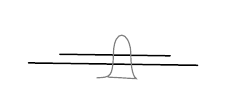
\begin{tikzpicture}[x=1mm,y=1mm,line cap=round]
\draw[line width=.19mm] (4,3)--(18,2.8) (0,1.9)--(21.5,1.6);
\draw[gray,line width=.15mm] (8.7,0).. controls (10.5,.1) and (10.7,.1)..(10.8,3.2)..controls (10.9,6.3) and (12.8,6)..(13,3.3)..controls (13,.8) and (13.4,.1)..(13.7,-.1)--(10.1,.1);
\end{tikzpicture}}
